%!TEX root=../document.tex

\section{Einleitung}
\subsection{Definition}
Replikation (lateinisch \textit{replicatio} \cite{duden} ``Wiederholung``, ``kreisförmige Bewegung``) \cite{dict} ist ``ein Verfahren der Datensicherung bei dem dieselben Daten von einem primären Speichermedium auf ein oder mehrere sekundäre Speichermedien kopiert werden.`` \cite{itw}

Demnach wäre Replikation also nichts anderes als ein simples Backup. Replikation wird jedoch besser definiert als mehrfache Speicherung \textbf{identer} Daten (an unterschiedlichen Orten) inklusive der Synchronisation selbiger. \cite{wiki}

Zwar gibt es inkrementelle Backups, die ebenfalls eine gewisse Synchronisierung der Daten beinhalten, jedoch erfolgt diese bei Backups stets einseitig. Bei der Replikation kann sie auch bidirektional implementiert werden. Ebenfalls wird bei einem Backup nie direkt mit den Sekundärdaten, also dem eigentlich Backup, gearbeitet, diese dienen lediglich als Absicherung im Verlustfall.

\subsection{Caching vs. Replikation}

Caching (Cache = Versteck, geheimes Lager) wird, im Unterschied zur Replikation, definiert als \textbf{temporäres} Speichern von redundanten Daten, die dynamisch ausgewählt werden. Zusätzlich sollte der Cache für die Administration möglichst unsichtbar sein, wovon bei der Replikation nicht die Rede sein kann. \cite{kaiserslautern}

\section{Pro \& Kontra}

\subsection{Gründe für Replikation}

Die Replikation ist also die bewusste Erzeugung redundanter Daten, obwohl dies eigentlich den Normalformen, die beim Planen einer Datenbank beachtet werden sollten, widerspricht. \cite{kaiserslautern} Trotzdem haben diese absichtlichen Redundanzen Vorteile:

\subsubsection{Skalierbarkeit}
\label{sec:scale}

Aufgrund mehrerer identer Datenbankinstanzen können Lesezugriffe verteilt werden. Somit wird die Last an den einzelnen Knoten reduziert und das Gesamtsystem wird dadurch leichter skalierbar. \cite{kaiserslautern}

\subsubsection{Verfügbarkeit}

Mithilfe von Replikation wird ebenfalls die Verfügbarkeit des Gesamtsystems erhöht, da im Fehlerfall eines einzelnen Knotens die Erreichbarkeit des Systems nicht beeinträchtigt wird. Andere Knoten können das System weiterhin aufrecht erhalten, womit der Extremfall ``Totalausfall`` ausgeschlossen wird. Zusätzlich gehen im Gegensatz zu einfachen verteilten Datenbanken keine Informationen verloren, sollte eine Instanz (dauerhaft) ausfallen, da alle Instanzen den identen Datensatz zur Verfügung haben. \cite{leipzig}

\subsubsection{Performance}

Replikation verbessert die Antwortzeiten auf zwei Arten:

Erstens werden die Antwortzeiten des Systems verkürzt, da die Last auf mehrere Server verteilt wird. Somit haben einzelne Knoten mehr Ressourcen zur Verfügung um einem Client schneller zu antworten. Das ist der angenehme Nebeneffekt der Skalierbarkeit (Unterpunkt \ref{sec:scale} auf Seite \pageref{sec:scale}). \cite{leipzig}

Zusätzlich werden die lokalen Antwortzeiten des Systems verkürzt, da stets auf eine ortsnahe oder netztopologisch günstige Instanz der Datenbank zugegriffen wird. \cite{leipzig}

\begin{figure}[!h]
	\begin{center}
		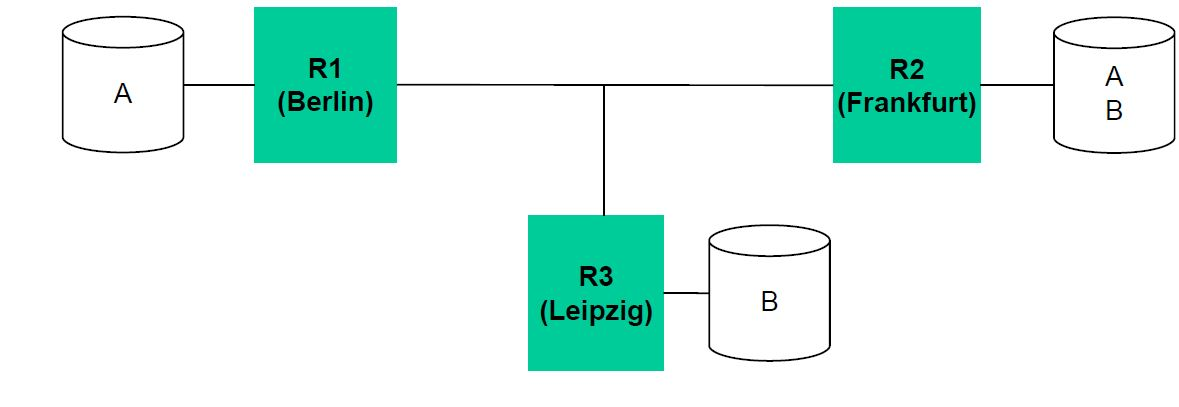
\includegraphics[width=1\linewidth]{images/ortsverteilung.jpg}
		\caption{Replikate an verschiedenen Standorten \cite{leipzig2}}
		\label{ortsvert}
	\end{center}
\end{figure}

Die verbesserten Antwortzeiten gelten meist nur für Lesezugriffe, da Schreibzugriffe in der Regel nicht vollkommen autonom ablaufen können. Dazu später mehr.

\subsubsection{Disconnected Computing}

Clients können ausgewählte Daten lokal replizieren, um damit später offline zu arbeiten. Im Anschluss müssen die Daten des lokalen Replikats mit den anderen Instanzen synchronisiert werden. \cite{leipzig} Die replizierten Daten sind in diesem Fall zwar meist nur temporär gespeichert, was eher auf die Funktion eines Caches hinweisen würde, jedoch wurden die zu replizierenden Daten im Vorhinein bewusst ausgewählt und im Anschluss werden sie wieder synchronisiert.

\subsection{Nachteile}

Für statische Daten sind die genannten Vorteile leicht mittels Replikation zu erreichen. Sollten sich die Daten ändern, müssen die Änderungen an alle Instanzen weitergegeben werden. Bei stark dynamischen Daten entstehen damit mehr Probleme, als gelöst werden. Deshalb wird Replikation typischerweise bei Stammdaten eingesetzt. \cite{kaiserslautern}
\clearpage
Durch die Synchronisation entstehen folgende Probleme:

\subsubsection{Aufwand}

Durch die benötigte Synchronisation der einzelnen Knoten wird das Netzwerk zwischen den Servern zusätzlich belastet. Eine Änderung an einem Knoten muss letztendlich an alle propagiert werden, weshalb der Rechenaufwand und die Netzauslastung bei stark dynamischen Daten schnell zum Problem werden.

\subsubsection{Speicherplatzbedarf}

Die vielen Instanzen benötigen insgesamt logischerweise mehr Speicherplatz, womit die Kosten für das Gesamtsystem wesentlich ansteigen. Aufgrund der Replikation ist die Menge der Informationen trotz erhöhten Speicherbedarfs gleich. Deshalb sollten die Gesamtsysteme so konzipiert werden, dass die zu replizierenden Daten der einzelnen Knoten sinnvoll ausgewählt werden.

Beispielsweise werden in der Zentrale in Frankfurt alle Datensätze benötigt. In Berlin benötigt eine andere Filiale derselben Firma nur einen Teil der Daten. In Leipzig wird wiederum nur ein anderer Teil der Daten benötigt (siehe Abbildung \ref{ortsvert} auf Seite \pageref{ortsvert}).

\subsubsection{Komplexität}

Mit der Anzahl der Knoten wächst auch die Komplexität des Gesamtsystems. Dadurch wird die Installation, Konfiguration und Wartung des Systems aufwendiger, was wiederum zu erhöhten Kosten führt.
\clearpage
\section{Anwendung}

Bei der Implementierung von Replikation gibt es im Prinzip drei Ziele, die miteinander im Konflikt stehen.

Das erste Ziel ist die Erhaltung der Datenkonsistenz. Dies kann entweder über eine \textbf{1-Kopien-Äquivalenz} \label{aequivalenz} oder eine kleine Kopienanzahl erreicht werden. Die 1-Kopien-Äquivalenz besagt, dass jeder Zugriff auf eine beliebige Instanz des Replikationsverbundes den neuesten konsistenten Zustand liefert. \cite{leipzig2} Das bedeutet, dass es möglichst zu jeder Zeit nur völlig idente Replikate gibt.

Das nächste Ziel, die Minimierung des Änderungsaufwands, wird ebenfalls durch eine kleine Anzahl von Kopien erreicht. Damit der Änderungsaufwand aber so gering wie möglich bleibt, sollen Replikate eher selten synchronisiert werden. \cite{leipzig2}

Der eigentliche Benefit der Replikation ist die Erhöhung der Verfügbarkeit und die Performance-Steigerung (vor allem) bei Lesezugriffen. Im Gegensatz zu den beiden anderen Zielen, wird dieses entweder mithilfe einer großen Anzahl an Kopien oder mit dem Zugriff auf beliebige, möglichst wenige Kopien erreicht. \cite{leipzig2} Letzteres erhöht jedoch nicht die Verfügbarkeit und kann nur implementiert werden, falls mehrere ortsnahe Knoten zur Verfügung stehen.

\begin{figure}[!h]
	\begin{center}
		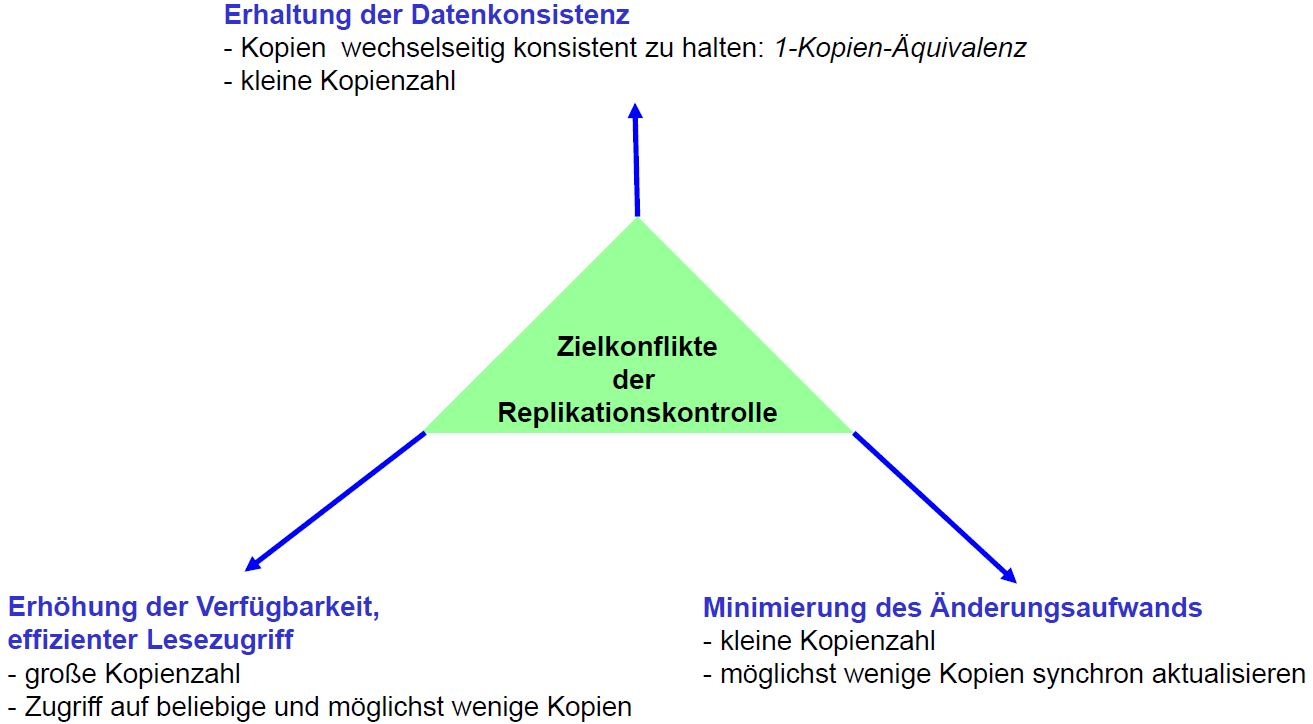
\includegraphics[width=1\linewidth]{images/konflikte.jpg}
		\caption{Zielkonflikte der Replikation \cite{leipzig2}}
		\label{konflikte}
	\end{center}
\end{figure}

\subsection{Mobile Computing}

\subsubsection{Szenario}

Für Außendienstmitarbeiter ist es wichtig, den Arbeitsort und die Arbeitszeit so flexibel wie möglich zu gestalten. Deshalb setzen Unternehmen zunehmend auf mobile Endgeräte. Aufgrund der Zeit- und Ortsflexibilität ist die Datenbank der Zentrale nicht ständig verfügbar. Damit die Endgeräte auch offline arbeiten können, müssen sie stets mit aktuellen, für den Mitarbeiter relevanten, Daten versorgt werden. Die benötigten Daten können je nach Termin variieren und werden daher täglich aktualisiert. In der Zentrale befindet sich die konsolidierte Datenbank aller Datensätze. \cite{kaiserslautern}

\subsubsection{Strategie}

Ausgewählte Datensätze der konsolidierten Datenbank werden also regelmäßig auf mobile Endgeräte repliziert. Finden auf den mobilen Endgeräten Änderungen statt, stellt sich die Frage, wie diese gespeichert werden. Nun gibt es zwei Arten dieses System zu implementieren. Entweder sind die replizierten Daten reine Lesekopien und Änderungen werden nur lokal gespeichert, d.h. es können keine Verkäufe oder ähnliche Schreibzugriffe getätigt werden. Ein andere Möglichkeit wäre es, das System bei erneuter Konnektivität zu synchronisieren. \cite{leipzig}

Dabei ist das Hauptziel die Erhöhung der Verfügbarkeit, die über eine hohe Kopienanzahl erreicht wird. Die Erhaltung der Datenkonsistenz ist bei dieser Art von Daten (Kundenstammdaten) leicht einzuhalten, da sie recht statisch sind. Der Änderungsaufwand ist ebenfalls gering, falls nur Lesezugriffe stattfinden. Die Endgeräte werden einfach täglich aktualisiert und arbeiten den restlichen Tag mit dem gleichen Datensatz. Kompliziert wird es jedoch, wenn die Synchronisation beidseitig funktionieren soll. Mit den Schreibzugriffen wird es schwieriger die Daten konsistent zu halten, da bei \textit{n} Endgeräten am Ende des Tages \textit{n} verschiedene Replikate vorhanden sind. Werden diese am Ende des Tages synchronisiert kann dies einen erheblichen Änderungsaufwand verursachen.

\subsubsection{Vorteile durch Replikation}

Diese Szenario wäre ohne Replikation nur mit einer zentralen Datenbank bewältigbar. Dadurch fehlt aber die Möglichkeit offline zu arbeiten, was auch der größte Vorteil der Replikation in diesem Szenario ist. Zusätzlich ist die Antwortzeit bei einer zentralen Datenbank wesentlich höher. \cite{kaiserslautern}

\subsection{Skalierbarkeit von Leselast}

\subsubsection{Szenario}

Webseiten verarbeiten täglich bis zu mehrere Millionen Anfragen. Bei diesen Anfragen handelt es sich bei ca. 97 - 99\% um Lesezugriffe. \cite{kaiserslautern} Einzelne Server sind logischerweise nicht in der Lage diese Vielzahl an Zugriffen zu verarbeiten. Deswegen setzt man einen Lastverteilungsverbund ein, in dem die Anfragen auf einzelne Knoten verteilt werden. Somit wird das Gesamtsystem auch für viele gleichzeitige Lesezugriffe einsetzbar.

\subsubsection{Strategie}

Es gibt also einen Serverbund aus möglichst identen Datenbanken, um die Vielzahl der Zugriffe aufzuteilen. Üblicherweise gibt es in diesen Konfigurationen einen Master-Server, auf dem auch Änderungen (Aktualisierungen der Informationen) durchgeführt werden können. Alle anderen Knoten sind Slave-Kopien, welche die Daten vom Master-Server erhalten. Auch hier werden Daten eingesetzt, die eher statisch sind.

Das Hauptziel ist hier die Skalierbarkeit, also die Lastverteilung. Diese wird durch eine mittlere - hohe Anzahl an Kopien erreicht, auf die möglichst wahlfrei zugegriffen werden kann. Da die Daten recht statisch sind, ist es ein leichtes, diese konsistent zu halten. Der Änderungsaufwand bleibt dadurch ebenfalls gering. Würde es sich um stark dynamische Daten handeln, würde der Änderungsaufwand und die fehlende Konsistenz den eigentlichen Nutzen der Replikation übersteigen.

\subsubsection{Vorteile durch Replikation}

Dieses Szenario wäre anders nur bewältigbar, wenn jeder Server verschiedenste Aufgaben erledigt und das System somit die Last verteilt, ohne teilweise redundant zu sein. Das Problem dieser Implementierung ist, dass die Aufgaben nicht immer gerecht geteilt werden und die Nutzungshäufigkeit der einzelnen Aufgaben nicht vorhergesehen werden kann.

\subsection{Hochverfügbarkeit}

\subsubsection{Szenario}

Viele Dienste müssen rund um die Uhr verfügbar sein und verwalten deshalb redundante Serverkopien. Fällt ein einzelner Knoten aus, so kann der nächste übernehmen.

\subsubsection{Strategie}

Dies könnte mit der vorhin beschriebenen Master/Slave Konfiguration mit vielen Slave Kopien gelöst werden. Wie bereits beschrieben, ist dieses Prinzip nur für statische Daten rentabel. Ändern sich die Daten sehr häufig, ist es sinnvoll die Anzahl der Slave Kopien zu reduzieren. Ansonsten ist der zu betreibende Änderungsaufwand zu hoch. Im Extremfall sollte mit einer einzelnen Slave Kopie gearbeitet werden, um den Synchronisierungsaufwand zu reduzieren. \cite{kaiserslautern} Damit die Performance des Systems nicht beeinträchtigt wird, werden die durchzuführenden Änderungsanweisungen an den Slave geschickt, der im Prinzip dieselben Aufgaben etwas zeitversetzt abarbeitet. Würden beide Server bei jeder Transaktion synchronisiert werden, würde die Bearbeitungszeit einer Anfrage wesentlich erhöht werden.

Das Hauptziel ist also die erhöhte Verfügbarkeit, die bei statischen Daten über eine große Kopienanzahl realisiert werden kann. Sind die Daten dynamisch, wird die Anzahl der Kopien eingeschränkt. Die Daten sollten so konsistent wie möglich sein, da der Hauptserver jederzeit ausfallen kann. Der Änderungsaufwand wird gering gehalten, indem eine Master/Slave Konfiguration eingesetzt wird.

\subsubsection{Vorteile durch Replikation}

Eine gewisse Ausfallsicherheit kann durch ein fehlertolerantes Design des Systems (USV, Notstromaggregat, usw.) erreicht werden. Ist beispielsweise aber die Serverhardware an sich defekt, so kann nur Redundanz und die damit verbundene Synchronisation der Schlüssel zum Erfolg sein.

\section{Asynchrone \& synchrone Replikation}

Abhängig von den oben genannten Zielen und Einsatzmöglichkeiten, kann die Replikation unterschiedlich implementiert werden. Der erste Unterschied zwischen einzelnen Implementierungen ist der Zeitpunkt der Synchronisation der Replikate.

\subsection{Synchrone Replikation}

Zugriffe auf Replikate sollten sich nicht von Zugriffen auf die Ursprungsdaten unterscheiden. Dies wäre der Fall, wenn eine \textbf{1-Kopien-Äquivalenz} (siehe Seite \pageref{aequivalenz}) gegeben wäre. Ein Weg zu diesem Ziel wäre die synchrone Replikation. \cite{darmstadt}

Hierbei werden alle Änderungen, die an einem Knoten vorgenommen werden, verzögerungsfrei auch an den anderen Knoten abgearbeitet. Somit gibt es jederzeit nur identische Kopien. Bevor also ein Schreibvorgang erfolgreich abgeschlossen ist, müssen alle Knoten des Systems den Vorgang bestätigen. Schlägt die Operation auf einem Knoten fehl, wird die Änderung auf allen Knoten rückgängig gemacht und die gesamte Transaktion ist fehlgeschlagen. \cite{leipzig}

\subsubsection{Vorteile}

Das ACID (Atomicity Consistency Isolation Durability) Prinzip wird mit synchroner Replikation weiterhin unterstützt. Jede Transaktion wird, für das Gesamtsystem gesehen, als atomare Einheit betrachtet. Man spricht auch von transaktionaler Konsistenz. \cite{kaiserslautern} Während der Änderung auf einem anderen Knoten werden Sperren auf den anderen eingesetzt, um ein eventuell gleichzeitiges Bearbeiten zu verhindern. Synchronisierungskonflikte können somit gar nicht erst entstehen. \cite{ralfb}

\subsubsection{Nachteile}

Sind alle Instanzen des Systems untereinander erreichbar, dann erhält man stets die neuesten Daten. Ist ein Teil des Verbunds aber nicht erreichbar, dann können veraltete Kopien entstehen. Meistens wird dies aber verhindert, indem Änderungen bei einem Teilausfall nicht möglich sind. \cite{kaiserslautern}

Somit wird auch die Verfügbarkeit des Systems beeinträchtigt. In einer solchen Konfiguration ist das Gesamtsystem nur erreichbar, wenn alle Teilsysteme erreichbar sind. Dies verschlechtert sogar die Verfügbarkeit des Gesamtsystems. Die Daten des Systems sind nur bearbeitbar, wenn in dem Moment keine Änderung stattfindet. Somit bringen mehrere Server keinen Benefit puncto Skalierbarkeit mehr.
\clearpage
Da auf die Rückmeldung aller Knoten gewartet werden muss, wird die Performance von Schreibzugriffen drastisch beeinflusst. \cite{kaiserslautern} Das Resultat dieser Einschränkung ist, dass synchrone Replikation nur über geringe Distanzen oder Hochleistungsnetzwerke verwendet werden kann. \cite{itw} Somit ist eine weltweite Verteilung auch nicht realisierbar.

\subsubsection{Einsatz}

Für mobile Computing ist synchrone Replikation also ungeeignet, da es hier um die Verfügbarkeit geht, die mit synchroner Replikation eher eingeschränkt wird. Die Hochverfügbarkeit wäre damit nicht möglich, da zu lange Wartezeiten entstehen und das Service damit wieder nicht verfügbar ist.

Bei eher statischen Daten kann die Leselast gut mit synchroner Replikation skaliert werden.

\subsection{Asynchrone Replikation}

Da die synchrone Replikation oft nicht möglich ist bzw. teilweise mehr Nachteile als Vorteile bringt, gibt es auch die asynchrone Replikation.

Hierbei werden Änderungen vorerst nur lokal vorgenommen. Damit das Datenbanksystem trotzdem noch die Forderung der Datenkonsistenz erfüllt, wird der Begriff Konsistenz durch \textbf{Konvergenz} ersetzt. Die Konvergenz stellt nur sicher, dass die Replikate nach einer gewissen änderungsfreien Zeit ident sind. \cite{kaiserslautern}

\subsubsection{Vorteile}

Da nicht auf das OK der anderen Knoten gewartet werden muss, reduziert die asynchrone Replikation die Antwortzeit bei Schreiboperationen drastisch gegenüber der synchronen Replikation. \cite{kaiserslautern}

Die Verfügbarkeit wird ebenfalls verbessert, da die Knoten auch bei Teilausfällen verfügbar sind.

\subsubsection{Nachteile}
\label{syncprob}

Bei verspäteter Synchronisierung der Datensätze kann es zu Konflikten kommen. Hierbei können Aktualisierungs-, Eindeutigkeits- und Löschkonflikte auftreten.

Bei Aktualisierungskonflikten wurde das gleiche Datenobjekt von unterschiedlichen Replikaten aus verändert. Nun muss entschieden werden, welche Version gültig ist. \cite{darmstadt}

Eindeutigkeitskonflikte betreffen das Einfügen von Datensätzen. Versuchen zwei Replikate ein Datenobjekt, mit dem gleichen Primärschlüssel oder anderen Daten die eindeutig sein müssen, hinzuzufügen, ergibt sich ebenfalls ein Konflikt. \cite{darmstadt}

Löschkonflikte entstehen, wenn der Datensatz auf einem Replikat gelöscht wird und auf einem anderen später noch bearbeitet wird. \cite{darmstadt}

Mit diesen Konflikten steigt der Updateaufwand erheblich an, es sei denn, die Konsistenz bzw. Konvergenz des Systems ist nicht von höchster Bedeutung.

\subsubsection{Einsatz}

Für dynamische Datensätze wird ausschließlich asynchrone Replikation eingesetzt.

Für mobile Computing eignet sich asynchrone Replikation perfekt, da die Außendienstmitarbeiter somit auch offline arbeiten können. Hochverfügbarkeit kann ebenfalls mit asynchroner Replikation gelöst werden, jedoch muss hier beachtet werden, dass Informationen verloren gehen, da die neuesten Änderungen im Fehlerfall noch nicht übertragen wurden.

Für die Skalierung reiner Leselast ist diese Art der Replikation ungeeignet, da die Replikate nicht konsistent sind und kein Performanceunterschied zur synchronen Replikation besteht.

\section{Unidirektionale \& bidirektionale Replikation}

Ein weiterer Unterschied zwischen den Implementierungsvarianten ist die Richtung der Synchronisation. 

\subsection{Unidirektionale Replikation}

Zur Skalierung der Leselast implementiert man einen Hauptserver, auf dem Änderungen durchgeführt werden können, und mehrere Nebenserver, auf denen Daten lediglich gelesen werden können. Dieses Master/Slave oder Publish-Subscribe Modell ist der Grundgedanke der unidirektionalen bzw. asymmetrischen Replikation.

\begin{figure}[!h]
	\begin{center}
		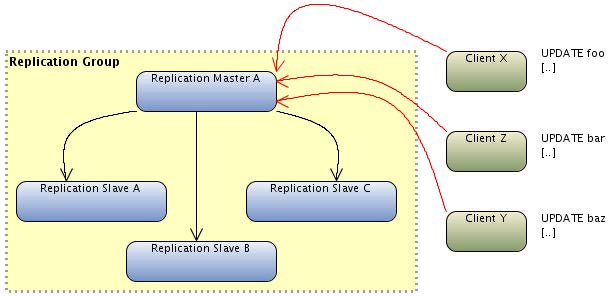
\includegraphics[width=1\linewidth]{images/unidirektional.jpg}
		\caption{Asymmetrische Replikation \cite{leipzig}}
		\label{unidirektional}
	\end{center}
\end{figure}

Hierbei werden alle Änderungen nur auf einer Instanz durchgeführt. Diese propagiert die Updates weiter und kümmert sich darum, dass die Slave-Server die aktuellen Daten erhalten. Auf die Nebenserver kann also nur für Leseoperationen zugegriffen werden. \cite{leipzig}

\subsubsection{Vorteile}

Der größte aber auch einzige Vorteil ist, dass keine Konflikte entstehen können. \cite{leipzig}

\subsubsection{Nachteile}

Die Rechenlast, für das Management der Synchronisation, liegt einzig und allein beim Master-Server. Darunter leiden vor allem die Skalierbarkeit und Verfügbarkeit des Gesamtsystems, da ein einzelner Server für eine Vielzahl an Schreiboperationen nicht ausreicht. 

\subsubsection{Einsatz}

Für mobile Computing ist unidirektionale Replikation eher weniger geeignet, da Außendienstmitarbeiter ihre Änderungen (Verkäufe) nicht durchführen können. Die Offline-Daten können lediglich für Produktinformationen und ähnliches verwendet werden.

Perfekt geeignet ist die asymmetrische Replikation für die Skalierung reiner Leselast.  Auch für Hochverfügbarkeit ist sie geeignet, da im Fehlerfall einfach ein Slave-Server die Rolle des Master-Servers übernehmen kann.

\subsection{Bidirektionale Replikation}

Da es auch Szenarien gibt, in denen der Schreibzugriff an mehreren Stellen sinnvoll ist, steht im Gegensatz zur asymmetrischen Replikation die bidirektionale.

\begin{figure}[!h]
	\begin{center}
		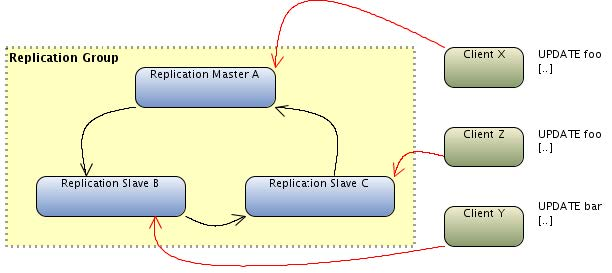
\includegraphics[width=1\linewidth]{images/bidirektional.jpg}
		\caption{Symmetrische Replikation \cite{leipzig}}
		\label{bidirektional}
	\end{center}
\end{figure}

Bei dieser Implementierungsvariante ist das Ändern von Datensätzen an jedem Knoten erlaubt. \cite{leipzig} Damit besitzt jedes Replikat die identen Schreib- und Leserechte.

\subsubsection{Vorteile}

Durch die mögliche Änderung an jeder Stelle können auch Schreibzugriffe skaliert werden. Dies geschieht durch eine Lastverteilung der Anfragen.

Ein gleichzeitiger Nebeneffekt ist, dass die Antwortzeit sinkt, da stets eine ortsnahe Kopie gewählt wird. Dies gilt logischerweise nur in Kombination mit asynchroner Replikation, da es ansonsten ständig Sperren gäbe.

\subsubsection{Nachteile}

Der Nachteil ist, dass hier wieder Konflikte entstehen können. Zwar könnte bidirektionale Replikation auch synchron implementiert werden, jedoch ist dies in der Praxis nicht der Fall. Aufgrund der asynchronen Replikation ergeben sich wieder die Synchronisierungskonflikte (siehe Seite \pageref{syncprob}). Deshalb ist abzuwägen, ob die Lastverteilung im Verhältnis zum gestiegenen Kommunikationsaufwand für die Synchronisierung rentabel ist. \cite{leipzig}

\subsubsection{Einsatz}

Für mobile Computing eignet sich die bidirektionale Replikation sehr, da somit auch offline produktiv gearbeitet werden kann.

In der Hochverfügbarkeit könnte man symmetrische Replikation entweder mit synchroner kombinieren und würde somit ein System erhalten, das für einzelne Anfragen lange Antwortzeiten hat und somit nicht mehr ständig verfügbar ist. Oder man kombiniert sie mit asynchroner Replikation, was im Fehlerfall einen erhöhten Informationsverlust zur Folge hätte, da die Änderungen noch nicht synchronisiert wurden. Für die Skalierung der Leselast eignet sich diese Strategie nicht, da sie keinen zusätzlichen Benefit dafür bringt.

\section{Klassifikation}

Tabellengrafik

Baumgrafik

\section{Resümee}
Replikation ist also...
Replikation ist gut wenn man folgendes beachtet...
gibt folgende Varianten ...